\documentclass[10pt]{article}
\usepackage[polish]{babel}
\usepackage[utf8]{inputenc}
\usepackage[T1]{fontenc}
\usepackage{amsmath}
\usepackage{amsfonts}
\usepackage{amssymb}
\usepackage[version=4]{mhchem}
\usepackage{stmaryrd}
\usepackage{graphicx}
\usepackage[export]{adjustbox}
\graphicspath{ {./images/} }

\title{Zadania - etap II (kl. II i III gimnazjum) }

\author{}
\date{}


\begin{document}
\maketitle
POLITECHNIKA GDAŃSKA

CENTRUM NAUCZANIA MATEMATYKI\\
I KSZTALCENIA NA ODLEGłOŚ̉

Zadanie 1. Jeżeli pewną liczbę dwucyfrową podzielimy przez sumę jej cyfr, to otrzymamy 4 i resztę 6 . Jeżeli natomiast liczbę tę podzielimy przez sumę jej cyfr pomniejszoną o 2 , to otrzymamy 5 i resztę 3. Znajdź tę liczbę.

Zadanie 2. Udowodnij, że suma kwadratów trzech kolejnych liczb naturalnych przy dzieleniu przez 3 daje resztę 2.

Zadanie 3. Koza i krowa zjadają razem wóz siana w ciągu 45 dni; krowa i owca - w ciągu 60 dni, zaś owca i koza w ciągu 90 dni. W ciągu ilu dni zjedzą wóz siana koza, krowa i owca razem?

Zadanie 4. Oblicz pole figury \(F\), ograniczonej wykresami funkcji:

\[
f(x):=|x|-2 \mathrm{i} \quad g(x):=2-|x|
\]

Zadanie 5. Oblicz długość przekątnej prostokąta \(K L M N\) o polu \(\frac{1}{2}\), wpisanego w kwadrat o boku długości 1, tak, jak na poniższym rysunku:\\
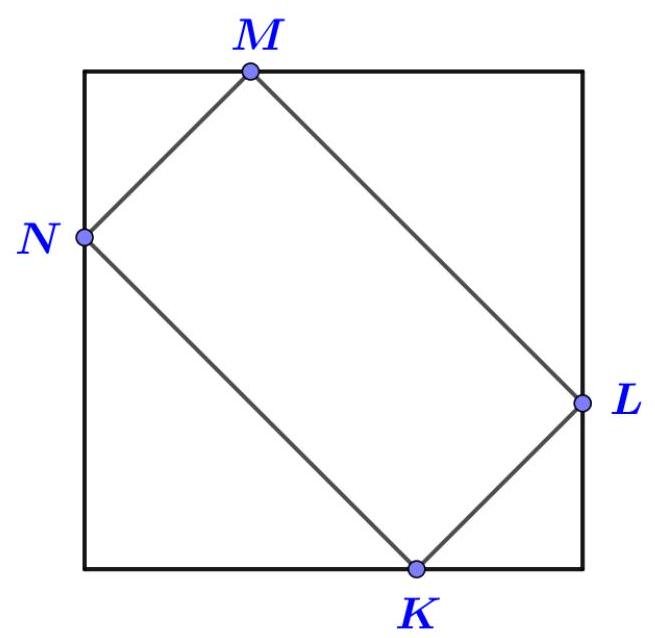
\includegraphics[max width=\textwidth, center]{2024_11_21_559aeed01947f67dd506g-1}


\end{document}